\documentclass[12pt]{article}

\usepackage{bm, graphicx, amssymb, amsmath, mathtools}
\usepackage[margin=1 in]{geometry}
\usepackage{mathtools}
\usepackage{epstopdf}
\usepackage{enumitem}
\usepackage{color}

\newcommand{\ds}{\displaystyle}
\newcommand{\B}[1]{{\bm #1}}
\newcommand{\U}[1]{{\hat{\bm #1}}}
\newcommand{\T}{^{\mbox{\tiny T}}}
\newcommand{\dd}{\; \text{d}}

%\thispagestyle{empty}

\begin{document}
	
	\newif\ifsolution    % Declaration, defaults to false
	
	%% Comment out this line to hide solutions
	%\solutiontrue
	
	\begin{center}{\bf AERO-222: Introduction to Aerospace Computation - Fall 2021\\ Homework \#2 - Due Date: Wednesday, October 6, 2021} \vspace{0.5cm}
		
		\textbf{\underline{Show all work and justify your answers!}} \vspace{0.5cm}
	\end{center}
	
	{\Large \textbf{Instructions}}
	\begin{itemize}
		\item \textit{This homework contains both handwritten and coding problems and shall be submitted according to the following guidelines.}
		\item \textit{Hardcopy:}
		\begin{itemize}
			\item \textit{Due on CANVAS at 11:59 PM on the day of the deadline.}
			\item \textit{Shall include screenshots of any hand-written work.}
			\item \textit{For coding problems, the hardcopy shall include any relevant derivations and emphasize the final results (i.e. boxed, highlighted, etc.).}
			\item \textit{Shall be submitted as a single file according to the provided template with the following naming scheme:} ``LastnameHW\#.pdf"
		\end{itemize}
		\item \textit{Coding Submission:}
		\begin{itemize}
			\item \textit{Due on CANVAS at 11:59 PM on the day of the deadline.}
			\item \textit{Shall be submitted as a single file according to the provided template with the following naming scheme:} ``LastnameHW\#.py"
			\item \textit{The script shall print out all outputs asked for in the problem}.
		\end{itemize}
		\item \textit{Late submissions will be accepted with a 10 point deduction per day late.}
	\end{itemize}
	\hrulefill
	
	\begin{description}
		%%%%%%%%%%%%%%%%%%%%%%%%%%%%%%%%%%%%%%%%%%%%%%%%%%%%%%%%%%%%%%
		\item[1. Newton's Method (15 pts) Code.] Apply the Newton method to find the root of the equation, $\sqrt{x+1} = e^{x} - 1$, using $x_0 = 0$ as an initial guess.
		\begin{enumerate}
			\item Report the final estimated error ($ \varepsilon_x$), {\bf not the residual}, of your solution using the prescribed residual tolerance: $| f(x_k) | < \varepsilon_y = 10^{-12}$. Report also the number of iterations. 
			\item Repeat the same problem, but stop the iterations when $| x_{k+1} - x_k | > | x_k - x_{k-1} |$ is satisfied. Report the number of iterations.
			\item Plot the convergence criteria as a function of iteration number from parts 1) and 2)
		\end{enumerate}
		
		\ifsolution
		\color{red}
		\textbf{Solutions:} \\
		\begin{equation*}
		\begin{cases}
		N_{\varepsilon_{y}} = 25 \\
		\varepsilon_{x} = \left|x_{k+1}-x_{k}\right| \approx 7.2141 \times 10^{-8} \\
		N_{\varepsilon_{x}} = 57
		\end{cases}
		\end{equation*}
		\color{black}
		\fi
		
		\item[2. Homotopy Continuation (10 pts) Code.] The Newton's method applied to find the root of the equation, $f (x) = 2x - 4 + \sin(2\pi x) = 0$, diverges if $x_0 = 0$ is selected as an initial guess. Solve this problem using homotopy continuation with step $\delta t = 0.025$. Provide subplots of the following as functions of $t$: (1) the number of iterations needed to converge at each step; (2) the estimated root. Use the residual tolerance $\varepsilon_y = 10^{-12}$ and $N_{\max} = 100$ as the maximum number of iterations.
		
		\ifsolution
		\color{red}
		\textbf{Solutions:}
		\begin{figure}[ht]
			\centering\includegraphics[scale=0.8]{HW2_Figs/HW2_P2.png}
		\end{figure}
		\color{black}
		\fi
		
		%%%%%%%%%%%%%%%%%%%%%%%%%%%%%%%%%%%%%%%%%%%%%%%%%%%%%%%%%%%%%%
		\item[2. Gaussian Elimination (15 pts) By-hand.] Use Gaussian Elimination with scaled partial pivoting to solve the following system of equations:
		\begin{equation*}
		\begin{cases}
		\begin{aligned}
		x_1 + 3x_2 + x_3 &= -1 \\ 
		2x_1 + 2x_2 - 6x_3 &= 2 \\ 
		3x_1 - x_2 + 2x_3 &= 3
		\end{aligned}
		\end{cases}
		\end{equation*}
		
		\ifsolution
		\color{red}
		{\bf Solution:}\\
		The system is first expressed as an augmented matrix:
		\begin{equation*}
		\left[
		\begin{array}{cccc }
		2 & 1 & -1 & -2 \\
		4 & 1 &  2 &  4 \\
		6 & 1 &  1 & 6 \\
		\end{array}
		\right]
		\end{equation*}
		Forward elimination: First, we swap rows 1 and 3:
		\begin{equation*}
		\left[
		\begin{array}{cccc }
		6 & 1 &  1 & 6 \\
		4 & 1 &  2 &  4 \\
		2 & 1 &  -1 & -2 \\
		\end{array}
		\right]
		\end{equation*}
		Multiply row 1 by 1/2 and subtract from row 2. Multiply row 1 by 1/3 and subtract from row 3.
		\begin{equation*}
		\left[
		\begin{array}{cccc }
		6 & 1 &  1 & 6 \\
		0 & 1/3 &  4/3 &  0 \\
		0 & 2/3 &  -4/3 & -4 \\
		\end{array}
		\right]
		\end{equation*}
		Swap rows 2 and 3:
		\begin{equation*}
		\left[
		\begin{array}{cccc }
		6 & 1 &  1 & 6 \\
		0 & 2/3 &  -4/3 & -4 \\
		0 & 1/3 &  4/3 &  0 \\
		\end{array}
		\right]
		\end{equation*}
		Multiply row 2 by 1/2 and subtract from row 3.
		\begin{equation*}
		\left[
		\begin{array}{cccc }
		6 & 1 &  1 & 6 \\
		0 & 2/3 &  -4/3 & -4 \\
		0 & 0 &  2 &  2 \\
		\end{array}
		\right]
		\end{equation*}
		Back substitution:
		\begin{equation*}
		\begin{split}
		& x_3 = \dfrac{2}{2} = 1 \\
		& x_2 = \dfrac{3}{2} \left(-4+4/3 \right)=-4 \\
		& x_1 = \dfrac{1}{6} (6-1+4) = 1.5
		\end{split}
		\end{equation*}
		\color{black}
		\fi
		
		
		%%%%%%%%%%%%%%%%%%%%%%%%%%%%%%%%%%%%%%%%%%%%%%%%%%%%%%%%%%%%%%
		\item[3. An Aerospace Application (15 pts) Code.] The following question brings together elements from multiple methods we've covered so far. An Airbus A320 is flying at Mach 0.7. It's Pitot tubes, shown in Figure \ref{fig:Pitot},  measure the total, or stagnation, pressure (pressure when the air hits and is stopped by the tube) as well as the static free-stream pressure.
		
		\begin{figure}[h!]
			\centering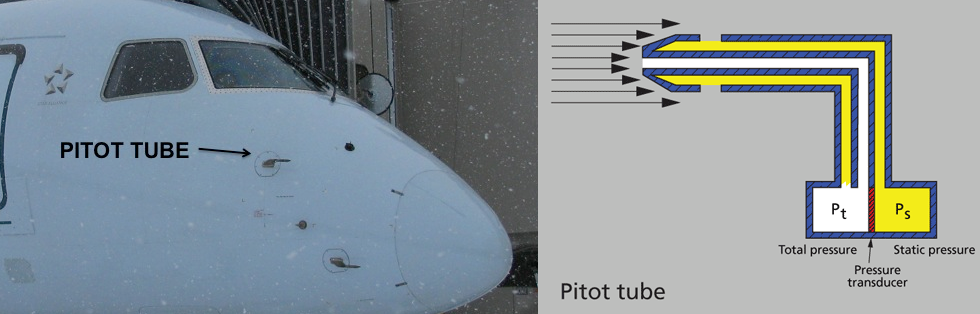
\includegraphics[width=4.5in]{HW2_Figs/pitot}
			\caption{Pitot-Static Tubes: Used to measure the ratio of total pressure to static pressure for determining aircraft airspeed.}
			\label{fig:Pitot}
		\end{figure}
		
		The ratio of total to static pressure is determined to be: $p_0/p = 1.289$. The following equation relates this change in pressure to the inlet Mach number, $M$, and $\gamma$, the heat capacity ratio:
		
		\begin{equation*}
		\frac{p_0}{p}= \left[ 1 + \frac{\gamma-1}{2}M^2 \right]^{\gamma/(\gamma-1)}
		\end{equation*}
		
		Based on the given pressure ratio and Mach number, determine the value of $\gamma$ that satisfies this equation to \emph{four significant figures} of accuracy. State what method you used, how many iterations it took and give your final solution estimate. \textbf{Hint:} Don't try to solve analytically for $\gamma$. It might be helpful to plot the function $f(\gamma)$ over a range of values to help you pick a good initial first guess. Choose from any of the iterative methods learned in class to solve.
		
		\ifsolution
		\color{red}
		\textbf{Solutions:}
		\begin{enumerate} [label=(\alph*)]
			\item 	
			First, rearrange the equation so that it equates to zero:
			\begin{equation*}
			f(k) = 0 = \left[ 1 + \frac{\gamma-1}{2}M^2 \right]^{\gamma/(\gamma-1)} - \frac{p_0}{p}
			\end{equation*}
			
			A few different methods are possible to find the root. Taking the derivative of this function with respect to $\gamma$ is complicated and so Newton's Method is not recommended, so one can try the Secant Method. I ended up using the bisection method to estimate my solution.
			
			\begin{figure}[ht]
				\centering\includegraphics[scale=0.5]{HW2_Figs/AERO222_HW2_P3.png}
				\caption{In order to establish the initial bracket, plot the function to see roughly where it crosses the x-axis}
				\label{fig:PitotPlot}
			\end{figure}
			
			Error Tolerance: $\varepsilon = 1 \times 10^{-5}$ \\
			Initial Steps: $x_{0} = 0, \ x_{1} = 0.1$ \\
			Given Parameters: $M = 0.7, \ p_0/p = 1.286$ \\
			
			\textbf{Results from Secant Method:}
			
			Number of Iterations = 3
			
			$x_{Secant} = 0.96498$
			
			$f(x_{Secant}) = -2.7110 \times 10^{-9}$
		\end{enumerate}
		\color{black}
		\fi
		
		%%%%%%%%%%%%%%%%%%%%%%%%%%%%%%%%%%%%%%%%%%%%%%%%%%%%%%%%%%%%%%
		\item[4. Fixed Point Iteration and Range of Convergence (10 pts) By-hand.] A fixed point is a point where $x = g (x)$. We will use fixed point iteration to find these points and then apply concepts from fixed point iteration in order to determine the range of convergence for root solving methods.
		\begin{enumerate} [label=(\alph*)]
			\item Given $x^2 -4x = 6x + 1$ give two functions, $g_1 (x)$ and $g_2 (x)$, for which we can perform fixed point iteration to solve for the roots of the equation above.
			\item Compute and draw the range of convergence (if any) on the interval $[-3,3]$ for both functions, $g_1 (x)$ and $g_2 (x)$.
		\end{enumerate}
		
		\ifsolution
		\color{red}
		{\bf Solution:}\\
		\begin{figure}[ht]
			\centering\includegraphics[scale=0.45]{HW2_Figs/HW12P2ab.png}
			\label{fig:5ab}
		\end{figure}
		\color{black}
		\fi
		
		
		%%%%%%%%%%%%%%%%%%%%%%%%%%%%%%%%%%%%%%%%%%%%%%%%%%%%%%%%%%%%%%
		\item[5. Newton's Method (20 pts) Code.] Given the function $f(x): -x^4 + 2x^3 = e^{-x} - 1$,
		\begin{enumerate} [label=(\alph*)]
			\item Find the root using Newton's method. Use $x_0 = 1.6$ and perform 5 iterations after the initial guess. Save the $x_k$ from each iteration to a vector.
			\item 	Determine if Newton's Method converges for the range of $x \in [-3,3]$ by using the convergence check for fixed point iteration. Provide a plot of $|g'(x)|$ to determine the range of convergence.
			\item Use the results from your code to provide a table of the estimated $x_k$ values from your Newton method iterations. Compute the order of convergence ($\alpha$) and the asymptotic error constant ($\lambda$) as accurately as possible using the $x_k$ values you have saved.
		\end{enumerate}
		
		\ifsolution
		\color{red}
		{\bf Solution:}\\
		\begin{enumerate} [label=(\alph*)]
			
			\item Applying the Newton Method, we obtain: \\
			\begin{equation*}
			\begin{cases}
			f(x) = -2x^3 + x - e^{-x} - 1 \\
			f'(x) = -6x^2 + 1 + e^{-x} \\
			x_{n+1} = x_k-\dfrac{f(x_k)}{f'(x_k)} \\
			x_k = [-2.0000, -1.6406, -1.5372, -1.5283, -1.5282, -1.5282]
			\end{cases}
			\end{equation*}
			\\
			
			
			\item Newton's Method converges when $x_{n+1} = x_k$ for $n \rightarrow \infty$. Therefore, if fixed point iteration converges when applied to Newton's Method, then Newton's Method must also converge.  Writing Newton's Method in the recursive form:
			\begin{equation*}
			x_{fpi} = g(x_{fpi}) = x_{fpi}-\frac{f(x_{fpi})}{f'(x_{fpi})}
			\end{equation*}
			
			Fixed point iteration converges for the interval $[a,b]$ if $|g'(x)| < 1$ for $x \in [a,b]$.
			
			\begin{equation*}
			|g'(x)| = \left| \frac{f(x)f''(x)}{(f'(x))^2} \right|
			\end{equation*}
			
			$f(x) = -2x^3 + x - e^{-x} - 1$ \\
			$f'(x) = -6x^2 + 1 + e^{-x}$ \\
			$f''(x) = -12x - e^{-x}$ \\
			
			Plugging this equation into Python and plotting, we can see that $\exists x \in [-3,3], \; |g'(x)| > 1 \implies$ FPI and the Newton Method are not guaranteed to converge on the interval [-3,3].
			
			\begin{figure}[ht]	\centering\includegraphics[scale=0.7]{HW2Figs/AERO222_HW2_P5.png}
				\caption{$\left|g'(x)\right|$ for $x \in \left[-3,3\right]$}
			\end{figure}
			
			\item The order of convergence and asymptotic error constant can be approximated as:
			
			\begin{equation*}
			\alpha= \frac{\ln e_{5}-\ln e_4}{\ln e_4 - \ln e_{3}} = 1.9977
			\end{equation*}
			\begin{equation*}
			\lambda= \dfrac{e_5}{e_{4}^\alpha} = 0.7989
			\end{equation*}
			
		\end{enumerate}
		\color{black}
		\fi
		
		%%%%%%%%%%%%%%%%%%%%%%%%%%%%%%%%%%%%%%%%%%%%%%%%%%%%%%%%%%%%%%
		\item[6. Order/Rate of Convergence (10 pts) By-hand.] By studying how the $x_k$ values generated by iterative methods change, we can see how quickly root solving methods converge.
		\begin{enumerate} [label=(\alph*)]
			\item What is the order of convergence, $\alpha$, for Newton's method? What if it's a tangential (double) root?
			
			\item For a linear method with an asymptotic error constant, $\lambda$, of 0.5 what is the ratio between successive errors (in $x$) after every iteration?
			
			\item Some really fast root solving method have cubic convergence with an asymptotic error constant $\lambda = 1/2$. Note $\lambda = \dfrac{e_k}{e_{k-1}^\alpha}$. If the initial error is $e_0 = 1$ give the error in fractional form for one, two, and three iterations.
		\end{enumerate}
		
		\ifsolution
		\color{red}
		{\bf Solutions:}  \\
		\begin{enumerate}[label=\alph*.]
			\item The ratio between successive error values is 1/2. The error reduces by 1/2 with every step.
			\item $\alpha = 2$. NM normally has quadratic convergence, however in the case of tangential root, it has linear convergence.
			\item $\alpha = 3$, $\lambda = 0.5$, $e_o =1$ \\
			we know $e_n/e_{n-1}^\alpha = \lambda$ b \\
			Therefore, $e_1 = \lambda e_{0}^\alpha = 0.5$ \\
			$e_2 = \lambda e_{1}^\alpha = 1/2^4 = 1/16 = 0.0625$ 
			$e_3 = \lambda e_{2}^\alpha = 1/2^13 = 1.221 \times  10^{-4}$ 
			
		\end{enumerate}
		\color{black}
		\fi
		
		\item[7. Aitken Acceleration (15 pts) Code.] Using Aitken acceleration with a fixed point, $E = g (E)$, solve Kepler's Equation: $M = E - e \, \sin E$, for a convergence tolerance defined as $|E_k - E_{k-1}| = 10^{-12}$. Assume $e = 0.65$, $M = \pi/16$, and the initial guess is $E_0 = M$. Compare the results obtained using Aitken acceleration to those obtained without Aitken acceleration. Plot the convergence of E both with and without Aitken acceleration.
		
		\ifsolution\color{red}
		\textbf{Solution:}
		Using Aitken Acceleration:
		\begin{equation*}
		\begin{cases}
		E = 0.385183461 \\
		N = 4
		\end{cases}
		\end{equation*}
		
		Without Aitken Acceleration (using nominal Fixed Point Iteration Method):
		\begin{equation*}
		\begin{cases}
		E = 0.385183461 \\
		N = 54
		\end{cases}
		\end{equation*}
		
		\fi	
		
	\end{description}
\end{document}

